% Drawing 154/02-22 -- folder 154, batch 02, archive page 35 (PDF page 36).
% Transcription: figure au bas de la colonne de gauche : quatre pseudo-droites orange issues d'un point $t$ et coupant une droite vert clair aux points $s_0$, $s_1$, $s_2$, $s_3$
% Kind: pencil of four lines through t cutting a line. Method 2 (schematic redraw from the facsimile). Status: ok.
% Notes: Four orange lines through t (one point), each through its marked point s_0, ..., s_3 of the light green line (points computed on the line); labels as on the page. Redrawn 2026-11-12 (issue 128): to check again.
% Coordinates: 1 unit = 1 mm = 1/100 of the crop width (bbox in page fractions: [0.13, 0.335, 0.27, 0.4]).
% Redrawn by Claude (claude-fable-5-2), issue #128, 2026-11-12; not checked by a human; not compiled (no TeX in the session).
% Rights: reproduces part of the work -- behind RENDER_TRANSCRIPTS, never published by itself.
\documentclass[tikz,border=3pt]{standalone}
\usepackage{amsmath,amssymb}
\usetikzlibrary{patterns,arrows.meta}
\tikzset{Or/.style={orange!90!black}, Lg/.style={green!60!black!70}, pencil/.style={black!45}, struck/.style={black!35}, mpt/.style={circle,draw,inner sep=1.3pt}, pt/.style={circle,fill,inner sep=0.9pt}, opt/.style={circle,draw,fill=white,inner sep=1.1pt}}
\begin{document}
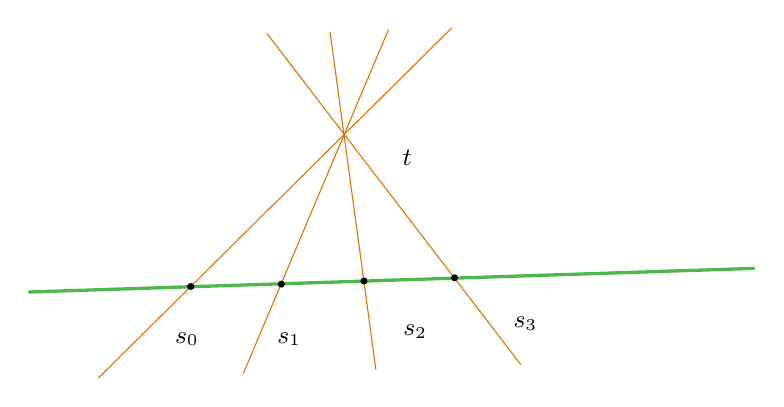
\begin{tikzpicture}[x=1mm,y=1mm,line cap=round,line join=round,font=\scriptsize]
\draw[Lg,very thick] (8,-47) -- (100,-44);
\draw[Or] (16.8,-57.9) -- (61.6,-13.5);
\draw[Or] (35.2,-57.3) -- (53.6,-13.7);
\draw[Or] (52,-56.8) -- (46.2,-14);
\draw[Or] (70.4,-56.2) -- (38.2,-14.2);
\node[pt] at (28.5,-46.3) {};
\node[pt] at (40,-46) {};
\node[pt] at (50.5,-45.6) {};
\node[pt] at (62,-45.2) {};
\node[inner sep=1pt] at (56,-30) {\small $t$};
\node[inner sep=1pt] at (28,-53) {\small $s_0$};
\node[inner sep=1pt] at (41,-53) {\small $s_1$};
\node[inner sep=1pt] at (57,-52) {\small $s_2$};
\node[inner sep=1pt] at (71,-51) {\small $s_3$};
\end{tikzpicture}
\end{document}
